\documentclass{flossiner}

\title{Test Article}
\author{Andrei J. Vukolov\affiliation{BMSTU}, Olga V. Egorova\affiliation{BMS}}
\authorrunning{A. Vukolov, O. Egorova}
\keywords{keyword1, keyword2, keyword3 (max. 5 values)}

\begin{document}
    \maketitle
    \begin{abstract}
    	%Use \hspace*{\fill} to omit stretching
    	Abstract comes here. 10pt. Max. 250 words\hspace*{\fill}
    \end{abstract}

\section{Introduction}
Introduction comes here. 12pt, regular, justified. Don’t use inline. Line-height=1.15, add space after paragraph. 

The document should link the \LaTeX\ class file \texttt{flossiner.cls} provided from the official website through following directive: \lstinline[language=TeX]|\documentclass{flossiner}|.

\section{Method}
\subsection{Sample or Study Group (second order title, 12pt, bold, italic)}
Please give detailed information here about your sample or study group.

\subsubsection{Tools \& \LaTeX\ prerequisites}
Class file \texttt{flossiner.cls} uses the following \LaTeX\ packages you should have on the machine to successfully compile the article:

	\begin{tabular}{ccc}
		\texttt{mathpazo}	&	\texttt{anyfontsize}	&	\texttt{ifthen}		\\
		\texttt{fancyhdr}	&	\texttt{geometry}		&	\texttt{graphicx}	\\
		\texttt{listings}	&	\texttt{color}			&	\texttt{hyperref}	\\
		\texttt{titlesec}	&	\texttt{tabularx}		&	\texttt{colortbl}	\\
		\texttt{environ}	&	\texttt{caption}		&	\texttt{apacite}
	\end{tabular}

All these packages are bundled into any modern \LaTeX\ distrubution. If you do not have one of them, you always can download it on CTAN: \href{https://www.ctan.org/}{https://www.ctan.org/}. Simply place the contents of uncompressed archive into the directory where \LaTeX\ would see it.

\section{Tables}
You may use centered \texttt{tabular} or unjustified \texttt{tabularx} environments wrapped into standard \texttt{table} floating object. Please keep the structure of your tables as simple and readable as possible.
\begin{table}[h]
	\caption{Sample table}
	\label{tbl:tbl1}
		\begin{tabularx}{\textwidth}{p{10cm}cXr}
			\hline
			Group	&	par1	&	par2	&	par3	\\
			\hline
			Group1	&	10		&	20		&	30		\\
			Group2	&	400		&	500		&	800		\\
			\hline
		\end{tabularx}
\end{table}

You can also add source code listings into your articles. To do so, you should use \texttt{lstlisting} environment. Source code which represents Table~\ref{tbl:tbl1} is printed in Listing~\ref{lst:lst1}.

\begin{lstlisting}[language=TeX,label=lst:lst1,caption={Code for floating table (from above)}]
\begin{table}[h]%Table environment
	\caption{Sample table}
	\label{tbl:tbl1}
	\begin{tabularx}{\textwidth}{p{10cm}cXr}
		\hline %Place data under the line
		Group	&	par1	&	par2	&	par3	\\
		\hline %Separator
		Group1	&	10		&	20		&	30		\\
		Group2	&	400		&	500		&	800		\\
		\hline
	\end{tabularx}
\end{table}
\end{lstlisting}

The header string for the listing above looks like \lstinline[language=TeX]|\begin{lstlisting}[language=TeX,label=lst:lst1,caption={Code for floating table (from above)}]|.


For another language like C++ just change the header of the environment: \lstinline[language=TeX]|\begin{lstlisting}[language=C++,label=lst:lstcpp,caption={Code}]|:
\begin{lstlisting}[language=C++,label=lst:lstcpp,caption={C++ code example}]
#include <iostream>
using namespace std;
int main(int argc, char** args)
{
	cout << "Hello World!" << endl;
	return 0;
}
\end{lstlisting}

\section{Figures}
To include images into your article please use standard \texttt{figure} environment wrapping \texttt{includegraphics} command as the following (fig.~\ref{fig:fig1}):
\begin{figure}[h]
	\begin{center}
		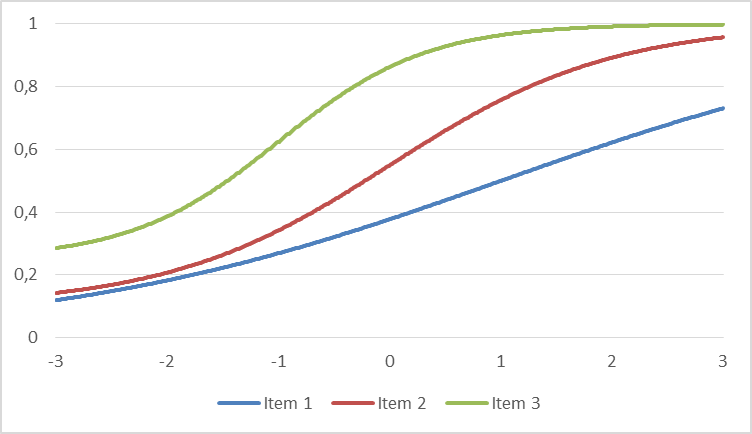
\includegraphics[width=0.75\textwidth]{testfigure}
		\caption{Test figure}
		\label{fig:fig1}
	\end{center}
\end{figure}
\begin{lstlisting}[language=TeX,label=lst:lst2,caption={Code for floating figure}]
\begin{figure}[h]
	\begin{center}
		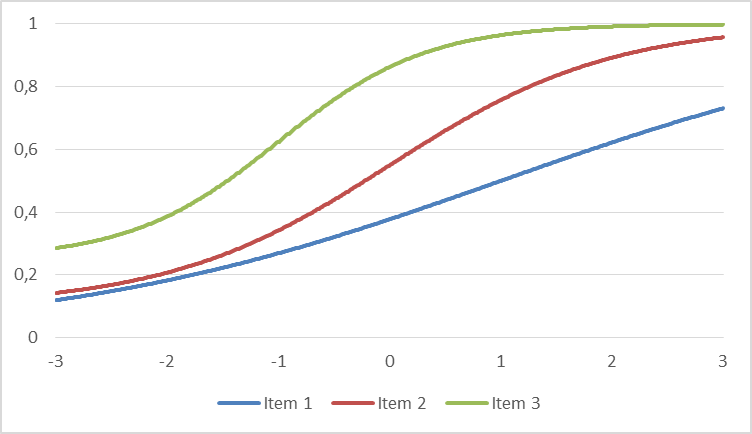
\includegraphics[width=\textwidth]{testfigure}
		\caption{Test figure}
		\label{fig:fig1}
	\end{center}
\end{figure}
\end{lstlisting}

\section{Conclusion}
You can edit this title as Summary, etc.

%\section{Suggestions}
%You can merge this title with Conclusion, or edit this title as Recommendations, etc.

\section{Acknowledgments}
Please provide any notes about your article (inc. grants, financial support etc.) under this section.

\section{Bibliography}
Use \texttt{apacite} bibliography style to generate citations using BibTeX. It is strongly unrecommended to write \lstinline[language=TeX]|\bibitem| commands manually because of very specific form of APA entry. Instead of it, use bibliographic entries collected within \texttt{.bib} file according to BibTeX documentation (\href{http://www.bibtex.org/}{http://www.bibtex.org/}) and write the following commands:
\begin{lstlisting}[language=TeX,caption={Adding a bibliography}]
	\bibliographystyle{apacite}
	\bibliography{books}
\end{lstlisting}
where \texttt{book} is the name of your \texttt{.bib} file. These commands will also add 'References' section automatically.

\end{document}
